\documentclass{ximera}



\begin{document}
\author{Alexander Holvoet}
\xmtitle{Lineaire combinaties, lineaire onafhankelijkheid en voortbrengend deel}{}

\subsection*{Inleiding}
Je bent een jonge reiziger die voor het eerst van huis gaat.
Je ouders willen je helpen op je reis, dus hebben ze je twee vervoersmiddelen gegeven: een hoverboard en een magisch tapijt.
Je ouders vertellen je dat zowel het hoverboard als het magische tapijt bepaalde bewegingsbeperkingen hebben:
\begin{itemize}
    \item Hoverboard: We duiden de beperking van de beweging van het hoverboard aan met de vector $\begin{pmatrix} 3\\ 1\end{pmatrix}$.
    Hiermee bedoelen we dat als het hoverboard één uur ``vooruit'' zou bewegen, het langs een ``diagonaal'' pad zou bewegen dat zou resulteren in een verplaatsing van 3 kilometer naar het oosten en 1 kilometer naar het noorden van zijn startlocatie.
    \item Magisch tapijt: We duiden de beperking van de beweging van het magische tapijt aan met de vector $\begin{pmatrix} 1 \\ 2 \end{pmatrix}$.
    Hiermee bedoelen we dat als het magische tapijt één uur ``vooruit'' zou bewegen, het langs een ``diagonaal'' pad zou bewegen dat zou resulteren in een verplaatsing van 1 kilometer naar het oosten en 2 kilometer naar het noorden van zijn startlocatie.
\end{itemize}

\subsection*{Open problemen}
\begin{exercise}
Je oom George stelt voor dat je eerste avontuur zou moeten zijn om de wijze man, Oude Man Gauss, te bezoeken.
Oom George vertelt je dat Oude Man Gauss 107 kilometer naar het oosten en 64 kilometer naar het noorden van je huis woont.\newline

Onderzoek of het mogelijk is om Gauss te bezoeken met de twee vervoersmiddelen.
Maak daarbij gebruik van een diagram, en gebruik gepaste vectornotatie om je redenering te ondersteunen.
\begin{hint}
Gauss' huis bevindt zich op de locatie die kan worden beschreven door de vector $\begin{pmatrix} 107 \\ 64 \end{pmatrix}$.
\end{hint}
\begin{hint}
Je kan de vervoersmiddelen ook achteruit gebruiken.
Als je \(h\) uren het hoverboard gebruikt en \(m\) uren het magische tapijt, dan is je verplaatsing gegeven door de lineaire combinatie:
\[h \begin{pmatrix} 3 \\ 1 \end{pmatrix} + m \begin{pmatrix} 1 \\ 2 \end{pmatrix} = \begin{pmatrix} 107 \\ 64 \end{pmatrix}\]
\end{hint}
\begin{oplossing}
Maak zelf een tekening om het grafisch te illustreren!\newline
Algebraïsch zoeken we coëfficiënten \(h\) en \(m\) zodat:
\[h \begin{pmatrix} 3 \\ 1 \end{pmatrix} + m \begin{pmatrix} 1 \\ 2 \end{pmatrix} = \begin{pmatrix} 107 \\ 64 \end{pmatrix}\]
Dit geeft het stelsel:
\[
\left\{
    \begin{array}{@{}l@{}}
    3h+m=107\\
    h+2m=64
    \end{array}
\right.
\]
wat oplossing \(h=30\), \(m=17\) heeft.
Gauss bezoeken is dus effectief mogelijk door 30 uur het hoverboard te gebruiken en 17 uur het magische tapijt.
(Maakt het uit in welke volgorde, of hoe je die 30 en 17 uur verdeelt?)
\end{oplossing}
\end{exercise}

\begin{exercise}
Gauss zou graag zijn hutje verplaatsen.
Je weet niet helemaal waarom, maar het betekent alleszins dat je niet zeker weet of je hem nog zal kunnen bezoeken...\newline

Zijn er plaatsen waar je Gauss niet kan bezoeken?
Beschrijf de plaatsen die je wel kan bezoeken, zowel geometrisch als algebraïsch, met behulp van een lineaire combinatie.
Maak ten slotte een overtuigend argument of er onbereikbare plaatsen zijn waar Gauss zich kan verstoppen.
\begin{hint}
    Gebruik opnieuw de lineaire combinatie van daarnet: \(h \begin{pmatrix} 3 \\ 1 \end{pmatrix} + m \begin{pmatrix} 1 \\ 2 \end{pmatrix}\)
    Welke waardes voor \(h\) en \(m\) zijn mogelijk?
\end{hint}
\begin{oplossing}
    Algebraïsch: alle bereikbare punten zijn van de vorm \(h \begin{pmatrix} 3 \\ 1 \end{pmatrix} + m \begin{pmatrix} 1 \\ 2 \end{pmatrix}\).
    Essentieel om in te zien is dat \(h\) en \(m\) ieder getal in \(\mathbb{R}\) kunnen zijn (positief, negatief, breuk, enzovoort).
    Als je punt \(\begin{pmatrix} x \\ y \end{pmatrix}\) wil bereiken, dan moet het stelsel
    \[
    \left\{
        \begin{array}{l}
        3h+m=x\\
        h+2m=y
        \end{array}
    \right.
    \]
    een oplossing hebben, en dat is altijd het geval.\newline

    Meetkundig kan je een tekening als in Figuur~\ref{fig:specificdisplaylinearcombo} maken, om te zien dat ieder punt in het vlak bereikt kan worden door een geschikte combinatie van de twee richtingen.
    \begin{figure}[H]
    \centering
    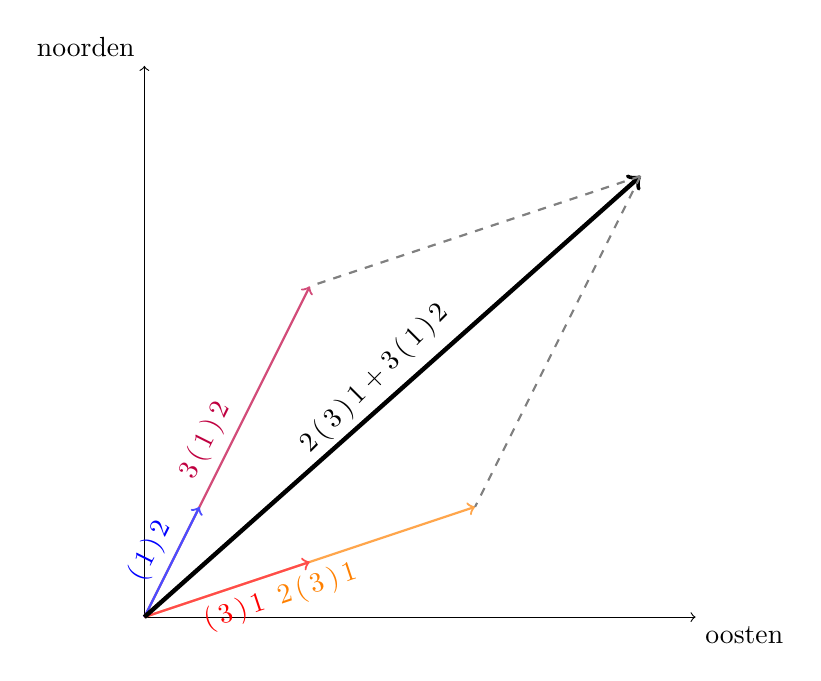
\begin{tikzpicture}[scale=0.7]

    \draw[->] (0,0) -- (10,0) node[below right] {oosten};
    \draw[->] (0,0) -- (0,10) node[above left] {noorden};

    % specifieke lineaire combinatie
    \draw[->, thick, orange!70] (0,0) -- (6,2) node[midway, below, sloped, black] {$\color{orange}2\begin{pmatrix} 3 \\ 1 \end{pmatrix}$};
    \draw[->, thick, purple!70] (0,0) -- (3,6) node[midway, above, sloped, black] {$\color{purple}3\begin{pmatrix} 1 \\ 2 \end{pmatrix}$};

    % basisvectoren hoverboard en tapijt
    \draw[->, thick, red!70] (0,0) -- (3,1) node[midway, below, sloped, black] {$\color{red}\begin{pmatrix} 3 \\ 1 \end{pmatrix}$};
    \draw[->, thick, blue!70] (0,0) -- (1,2) node[midway, above, sloped, black] {$\color{blue}\begin{pmatrix} 1 \\ 2 \end{pmatrix}$};
    
    % Resultant vector
    \draw[->, ultra thick,] (0,0) -- (9,8) node[midway, above, rotate=45, black] {$2 \begin{pmatrix} 3 \\ 1 \end{pmatrix} + 3 \begin{pmatrix} 1 \\ 2 \end{pmatrix}$};
    
    % Dashed projection lines
    \draw[dashed, gray, thick] (9,8) -- (6,2);
    \draw[dashed, gray, thick] (9,8) -- (3,6);
    \end{tikzpicture}
    \caption{Een voorbeeld van een lineaire combinatie van de hoverboard- en tapijtrichtingen.}
    \label{fig:specificdisplaylinearcombo}
    \end{figure}
    Formeel betekent dit dat de voortgebrachte verzameling van \(\begin{pmatrix} 3 \\ 1 \end{pmatrix}\) en \(\begin{pmatrix} 1 \\ 2 \end{pmatrix}\) het hele vlak \(\mathbb{R}^2\) is, oftewel:
    \[
    \text{span}\left\{\begin{pmatrix} 3 \\ 1 \end{pmatrix}, \begin{pmatrix} 1 \\ 2 \end{pmatrix}\right\} = \mathbb{R}^2
    \]
\end{oplossing}
\end{exercise}

\subsection*{Uitbreiding naar 3 dimensies}
Stel dat je nu in een driedimensionale wereld bent voor het gelijkaardige probleem, en je hebt drie transportmodi:
\[\mathbf{v}_1 = \begin{pmatrix} 1 \\ 1 \\ 1 \end{pmatrix}\quad \text{, }\mathbf{v}_2 = \begin{pmatrix} 6 \\ 3 \\ 8 \end{pmatrix}\quad \text{en }\mathbf{v}_3 = \begin{pmatrix} 4 \\ 1 \\ 6 \end{pmatrix}\]

Je mag ieder transportmiddel slechts \textbf{één keer} gebruiken voor een bepaalde duur \(t_1\), \(t_2\) en \(t_3\) (positief voor vooruit, negatief voor achteruit).
Laat ons bekijken wat dit nu verandert aan de plaatsen die je kan bereiken.

\begin{exercise}
Kan je een reis maken waarbij je thuis begint en ook eindigt?
Zo ja, vind \(t_1\), \(t_2\) en \(t_3\) zodat je terug thuis komt.
Zo nee, leg uit waarom niet.

\begin{question}
Is er meer dan één manier om een reis te maken die voldoet aan de hierboven beschreven vereisten?
(Met andere woorden, zijn er verschillende combinaties van tijden die je kunt besteden aan de transportmodi zodat je terug thuis komt?)
Zo ja, hoe?
\end{question}

\begin{question}
Is er ergens in deze 3D-wereld waar Gauss zich voor je zou kunnen verstoppen?
Zo ja, waar?
Zo nee, waarom niet?
\end{question}

\begin{question}
Wat is \(\text{span}\left\{\begin{pmatrix} 1 \\ 1 \\ 1 \end{pmatrix}, \begin{pmatrix} 6 \\ 3 \\ 8 \end{pmatrix}, \begin{pmatrix} 4 \\ 1 \\ 6 \end{pmatrix}\right\}\)?
En wat betekent dit in de context van de transportmodi?
\end{question}
\end{exercise}

\subsection*{Afsluiter of huistaak}
Vul de volgende tabel in met de gevraagde verzamelingen van vectoren.
Schrijf de strategieën op die je gebruikt om de voorbeelden te genereren.
\begin{table}[H]
\begin{tabular}{|p{4cm}|p{4cm}|p{4cm}|}
\hline
& \textbf{Lineair afhankelijke verzameling} & \textbf{Lineair onafhankelijke verzameling} \\
\hline
\textbf{Een verzameling van 2 vectoren in $\mathbb{R}^2$} & & \\
\hline
\textbf{Een verzameling van 3 vectoren in $\mathbb{R}^2$} & & \\
\hline
\textbf{Een verzameling van 2 vectoren in $\mathbb{R}^3$} & & \\
\hline
\textbf{Een verzameling van 3 vectoren in $\mathbb{R}^3$} & & \\
\hline
\textbf{Een verzameling van 4 vectoren in $\mathbb{R}^3$} & & \\
\hline
\textbf{Een verzameling van 1 vector in \(\mathbb{R}^2\)}  &  & \\
\hline
\end{tabular}
\end{table}
Schrijf ten minste 2 generalisaties die kunnen worden gemaakt uit deze voorbeelden en de strategieën die je hebt gebruikt om ze te construeren.

\end{document}
